%!TEX TS-program = xelatex
%!TEX encoding = UTF-8 Unicode
\documentclass[11pt, a4paper]{article}

\usepackage{fontspec, xunicode, xltxtra}
\defaultfontfeatures{Mapping=tex-text}
\setmainfont{Adobe Caslon Pro}
\setmonofont[Scale=MatchLowercase]{Monaco}
\setmathsf{Cambria Math}

\usepackage{paralist} % for better itemize and enumerate
% asparaenum, inparaenum, \begin{compactenum}[{Example} a)] etc.
% Also, items can be referenced via \label{} and \ref{}
%
\frenchspacing
\usepackage{natbib}
\bibpunct{(}{)}{;}{a}{,}{,}
\usepackage{gb4e}
\usepackage{wrapfig}

% my macros
\def\code{\texttt}
\def\tred{\texttt{TrEd}}
\def\seman{\texttt{SemAnn}}
\def\astst{$\ast$.st}
\def\sdata{s-data}
\def\stn{st-node}
\def\sn{s-node}
\def\tn{t-node}
\def\stf{st-file}
\def\sf{s-file}
\def\tf{t-file}
\def\mwe{MWE}
\def\Mwe{multi-word expression}
\newcommand\Sref[1]{Section~\ref{#1}}

\title{Thesis Notes}
\author{\textsc{Pavel Straňák}}

\begin{document}
\maketitle

%%%%%%%%%%
\section*{Motto}
\begin{tabular}{@{} lp{11cm} @{}} % @{} removes default spaces
Frasier: & ``How was your hunting trip?''\\
Martin: & ``Came home empty handed.''\\
Frasier: & ``Oh dear; I guess that means for the next several weeks we'll hear your grouse about the grouse and carp about the carp.''\\
Niles: & ``You've been working on that, haven't you?''\\
Frasier: & ``Well, there was traffic.''\\
 & \raggedleft\emph{Frasier, Season 9, Part 3}\\
\end{tabular}

\section*{Idioms}
Even ``non-compositional'' idioms are actually (originaly) metaphorical or methonymical.  Even though sometimes it is hard to see that. At other times a speaker may forget that rather straightforward metaphoric aspect:

\begin{quote}
Barack Obama accused his Republican rivals of stirring a controversy over a comment he made about putting “lipstick on a pig.” \emph{(NY~Times, 11.~September 2008)}
\end{quote}


%%%%%%%%%%%%%%%%%%%%%%%%%%%%%%%%%%%%%%%
\section{PDT 2.0}\label{PDT}
In PDT there are several functors that refer to multiword expressions (MWEs) in one way or another. There are also some technical lemmas (??? nebo jen 1?) like {\tt \#Forn} that identify roots of subtrees representing MWE's.

There are currently two graphical search engines for PDT: Netgraph \cite{netgraph} and TrEd \cite{tred}. Both have their respective benefits, but since TrEd is considerably faster due to its use of an SQL database backend \cite{pmltq}, we have used TrEd for all the examples in this work. We also give the search queries using the PML Tree Query language \cite{pmltq} where appropriate.

%%%%%%%%%%
\subsection{Foreign Phrase: \code{t-node [t\_lemma = \#Forn]}}\label{PDT:Forn}
Foreign Phrase seems to be overused and its overuse seems a bit arbitrary. \\
- jmena firem jsou nekdy forn, nekdy ne. (dohledat)\\

%%
\subsubsection{Foreign phrases with just one t-node}
There are 34 occurrences of this construction in the PDT~2.0. Counting them is as easy as writing a query in Figure~\ref{fig:tq-forn1} and extending it with this filter: \code{>>count(\$n)}.

\begin{wrapfigure}{r}{0.32 \textwidth}
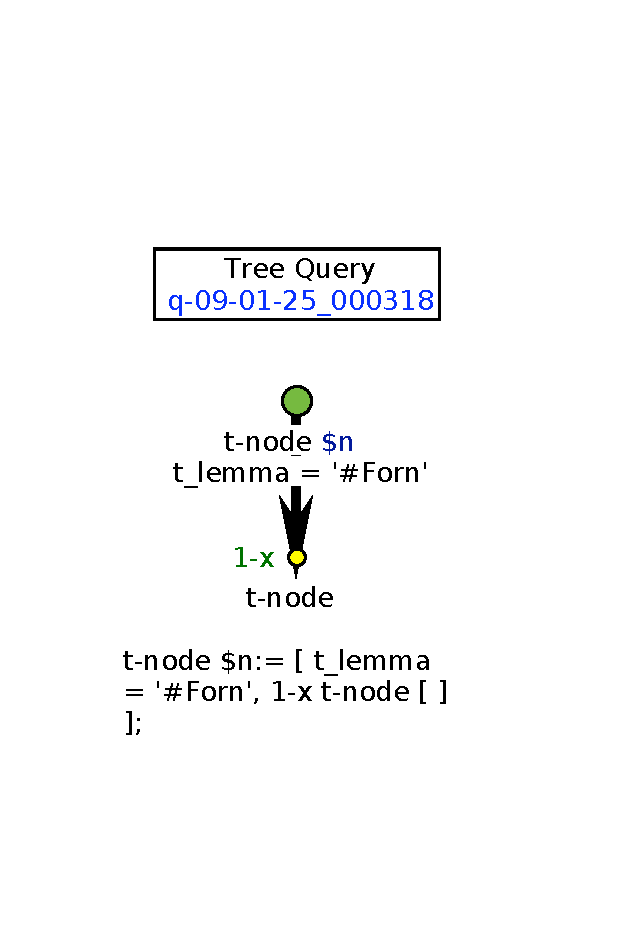
\includegraphics[width=0.3 \textwidth]{images/vyhledavky/query-forn-1-x.pdf}
\caption{PML-TQ search query for single-node foreing phrases}
\label{fig:tq-forn1}
\end{wrapfigure}

In case of the bibliographic reference in Figure~\ref{fig:forn-biblio} there is coordination of three foreign phrases corresponding to the parts of a bibliographic reference annotated, but the reason for this is not very clear. After all, the point of annotating foreign phrases as simple lists with a \code{\#Forn} node as a head was to make no assumptions about these pieces of a text \pageref{pdt-t-man:300}.  \\
- je to kvuli te interpunkci???

\begin{figure}[h]
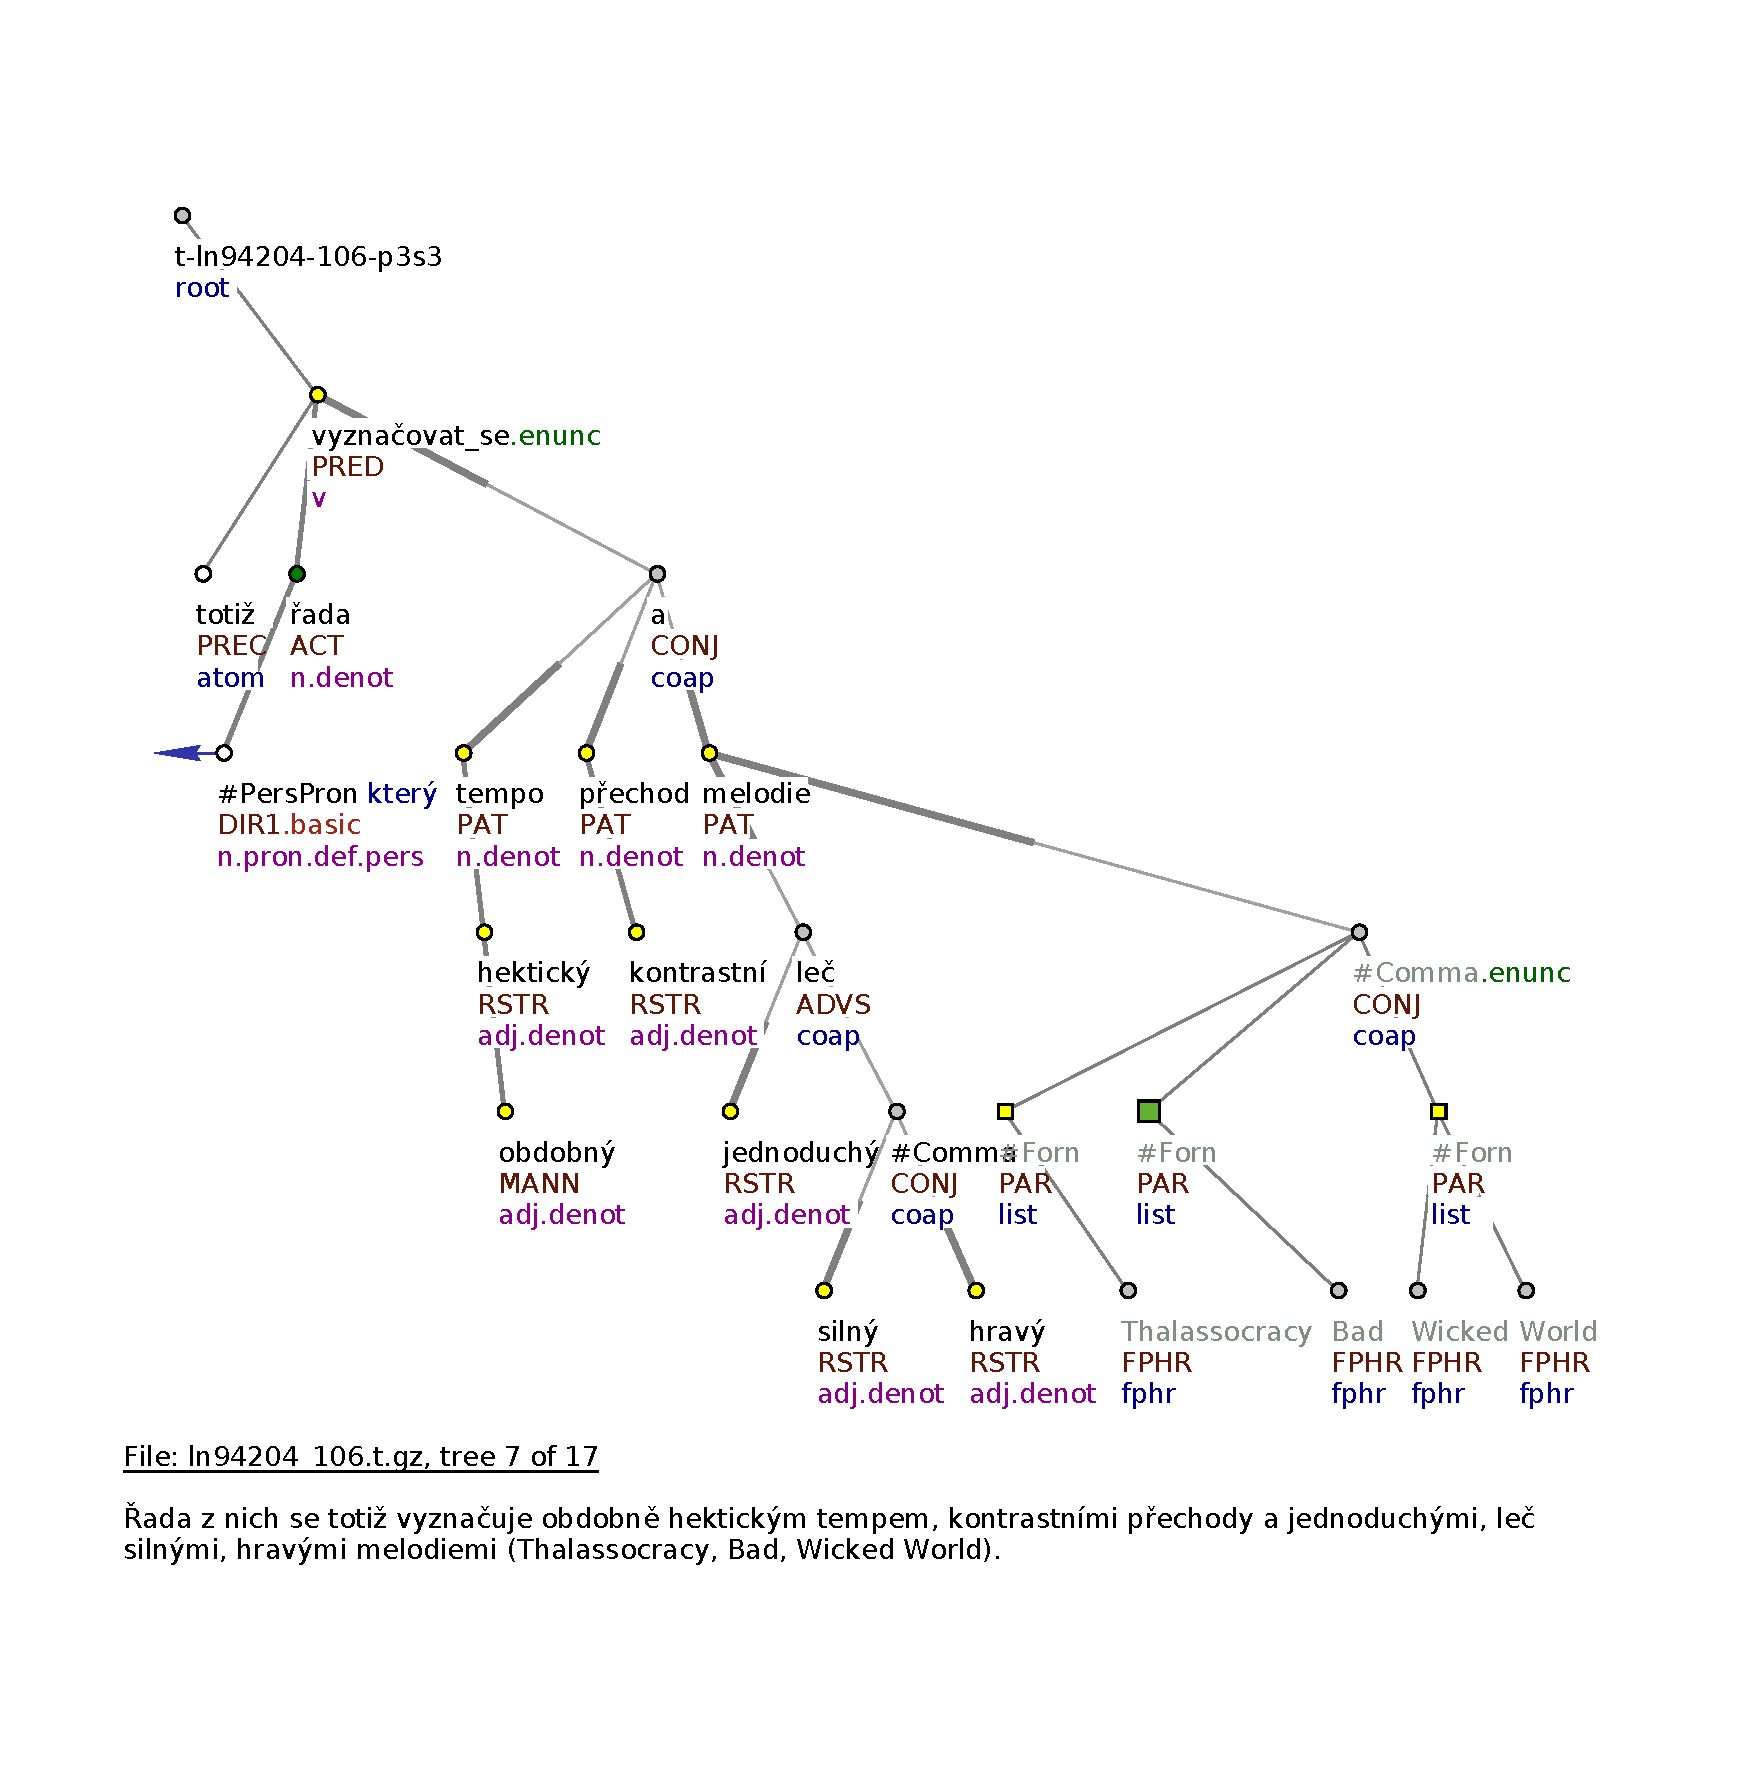
\includegraphics[width=\textwidth]{images/vyhledavky/forn-coord1x-biblio.pdf}
\caption{A bibliographic reference analysed as a coordination of three foreign phrases}
\label{fig:forn-biblio}
\end{figure}

Names of companies seem to be distinguished more by the country of origin then by any linguistic reasons, as demonstrated in Figure~\ref{fig:forn-firmy}. As far as linguistic criteria are concerned, Chemapol and Inekon are as foreign as Agip or Total. However the first two are, or at least were%
\footnote{At the time of writing this thesis Chemapol is owned by another international company, which only emphasises vagueness of this distinction} %
%
, Czech companies, while those in the latter group have a foreign origin.

\begin{figure}
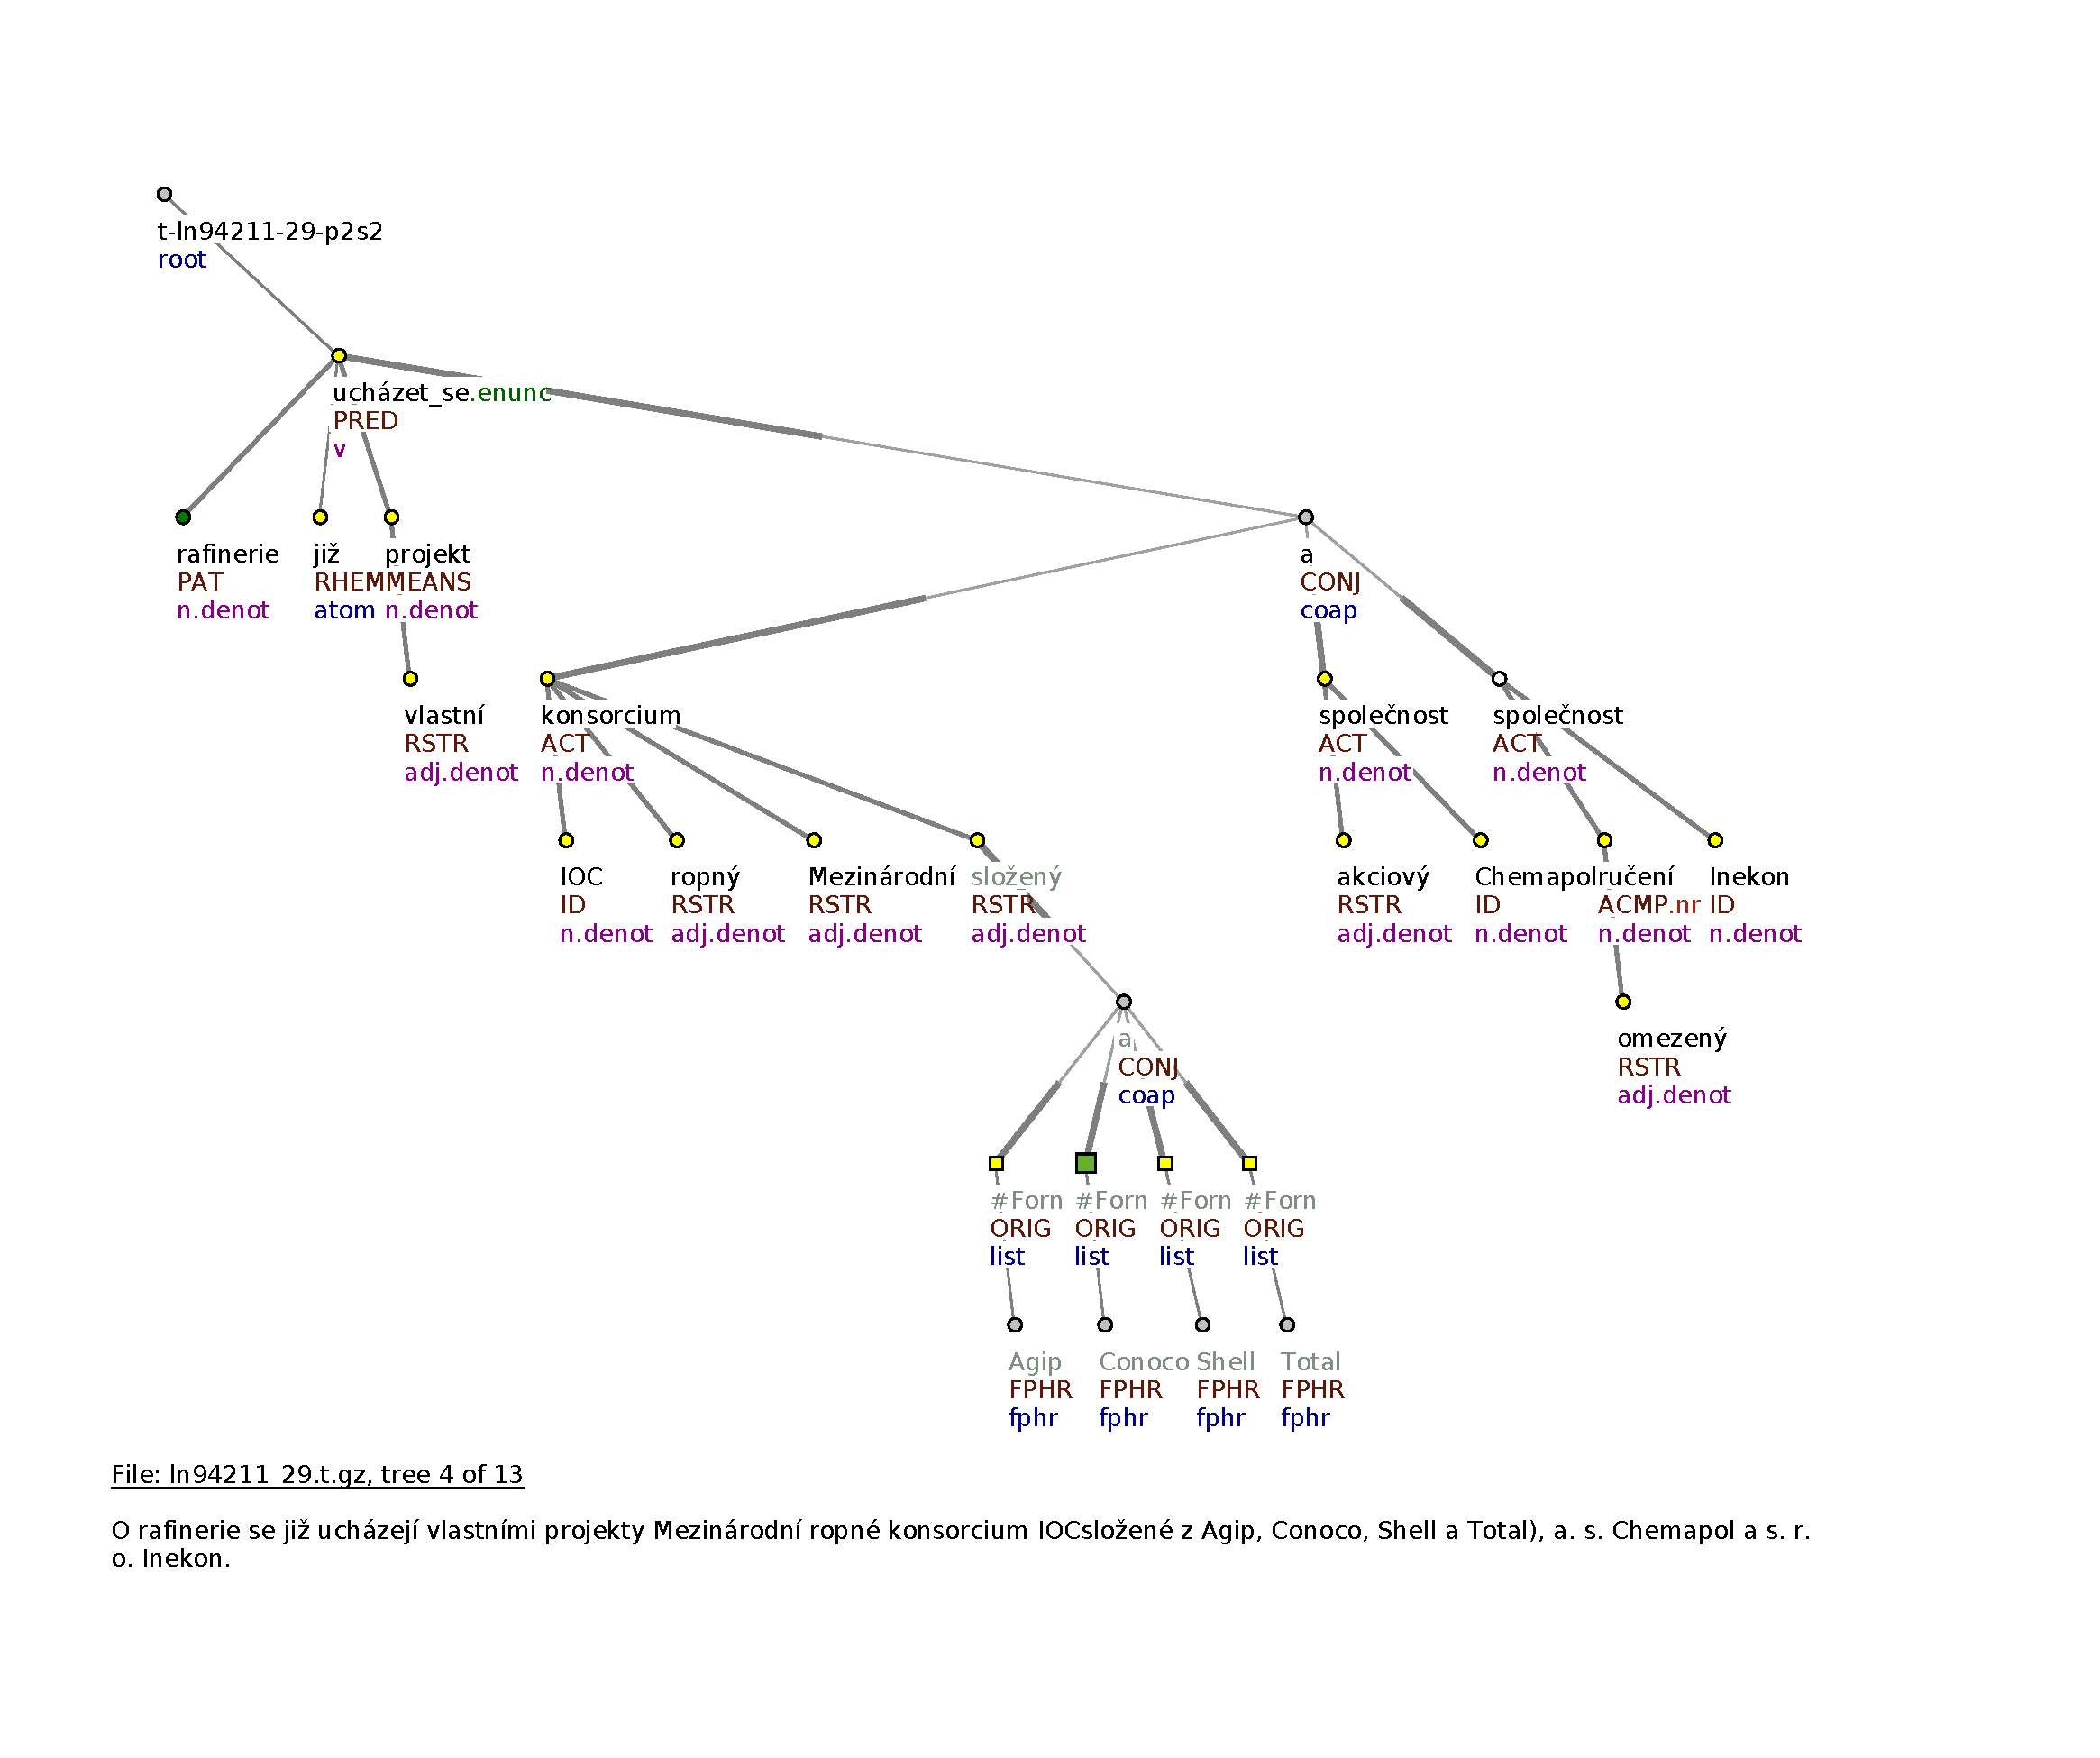
\includegraphics[width=\textwidth]{images/vyhledavky/nazvy-firem.pdf}
\caption{Annotation of Czech and foreign company names}
\label{fig:forn-firmy}
\end{figure}

%%%%%%%%%%
\subsection{CPHR}
There are 76 occurrences of {\tt CPHR} nodes, whose head verb is not its parent, but only effective parent, in 40 sentences. See Figure~\ref{fig:tq-echild} for the query and Figures~\ref{fig:cphr-echild} and~\ref{fig:cphr-echild2} for examples.
\begin{wrapfigure}{r}{0.32 \textwidth}
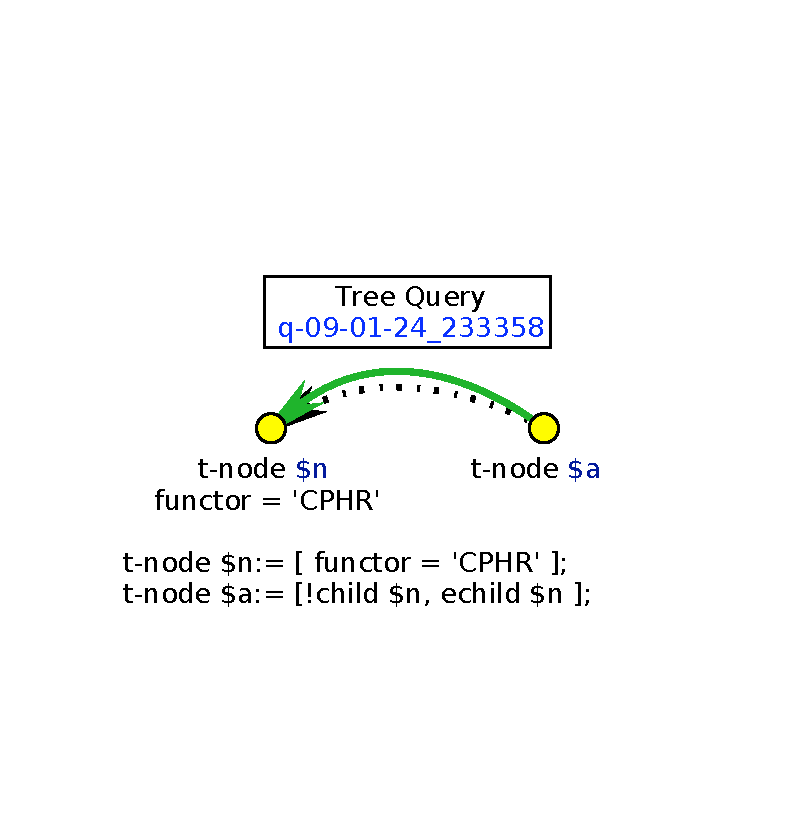
\includegraphics[width=0.3 \textwidth]{images/vyhledavky/query-echild.pdf}
\caption{PML-TQ search query for CPHR nodes, whose effective parrent is not its parent}
\label{fig:tq-echild}
\end{wrapfigure}

\begin{figure}[h]
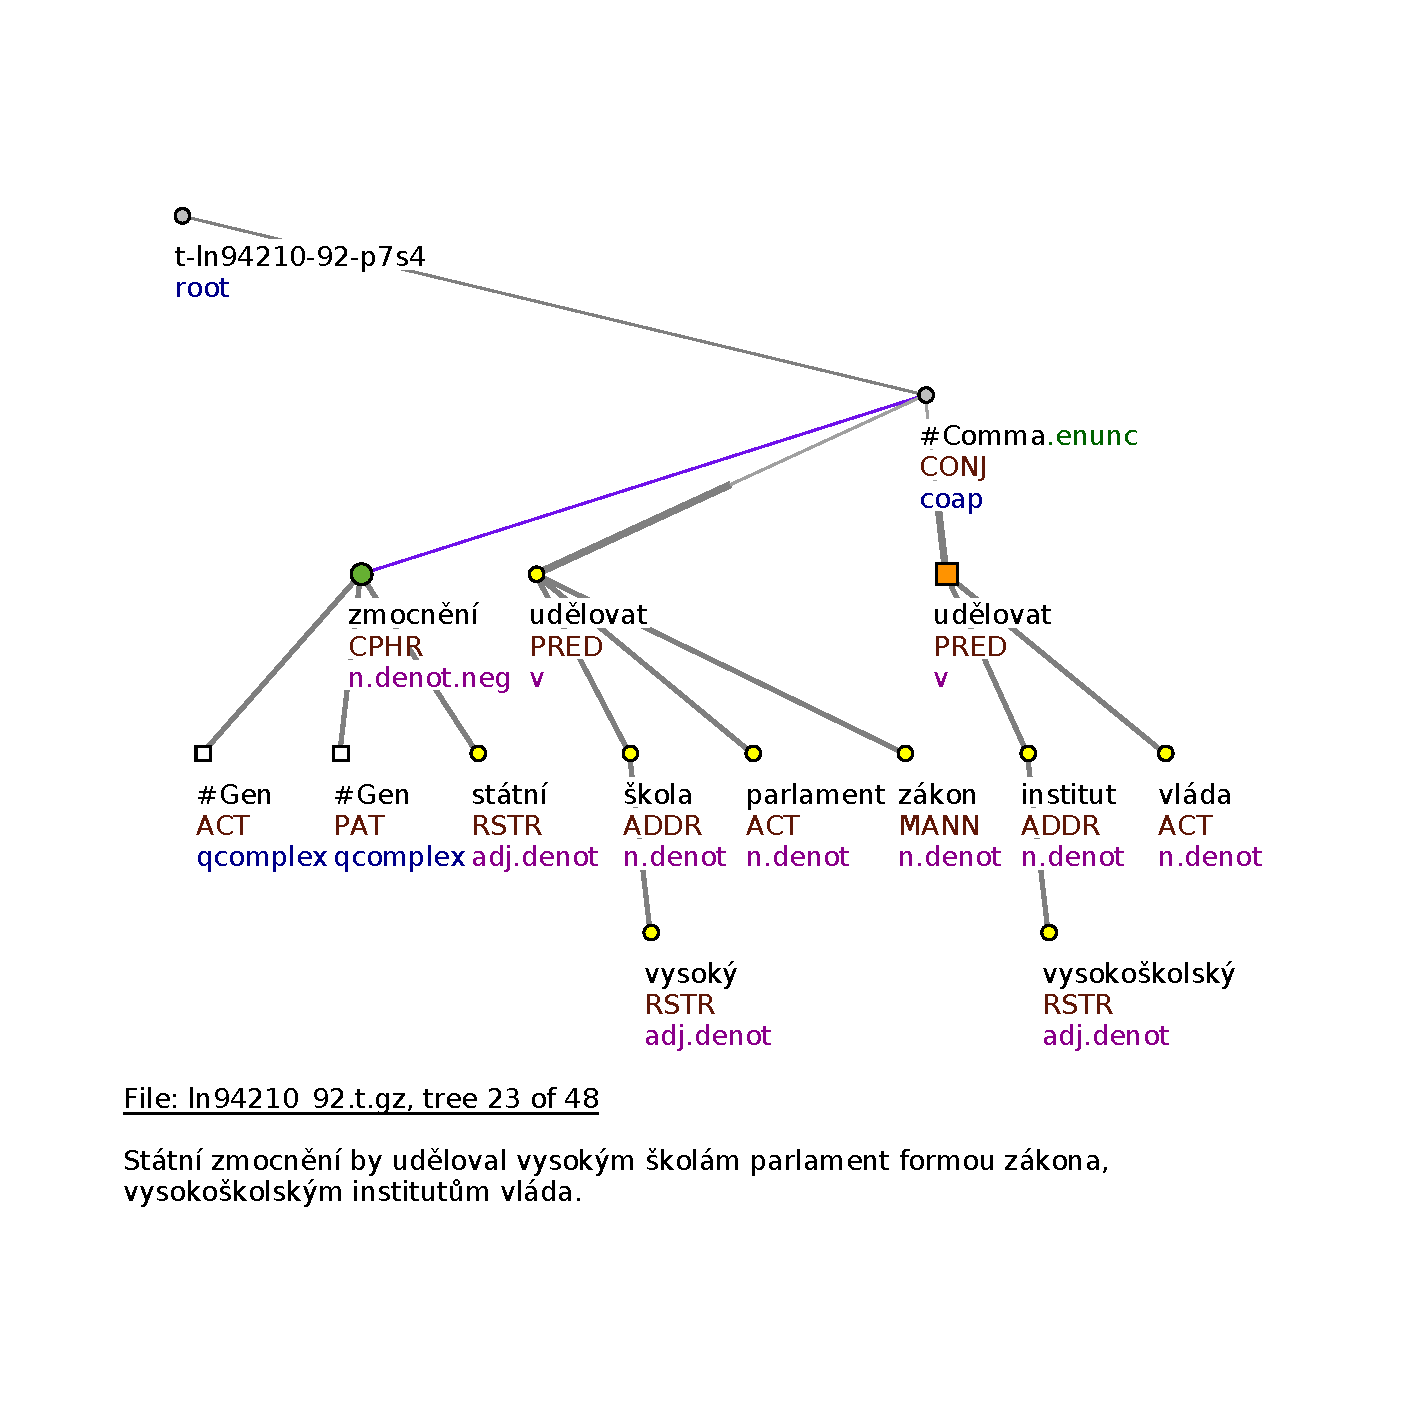
\includegraphics[width=0.8\textwidth]{images/vyhledavky/cphr-echild.pdf}
\caption{Coordination of verbonominal idioms, where the verbal parts are further ???rozvite }
\label{fig:cphr-echild}
\end{figure}

Figure~\ref{fig:cphr-echild2} shows on the other hand a coordination of two V-N idioms with the same verbal part.
\begin{figure}[h]
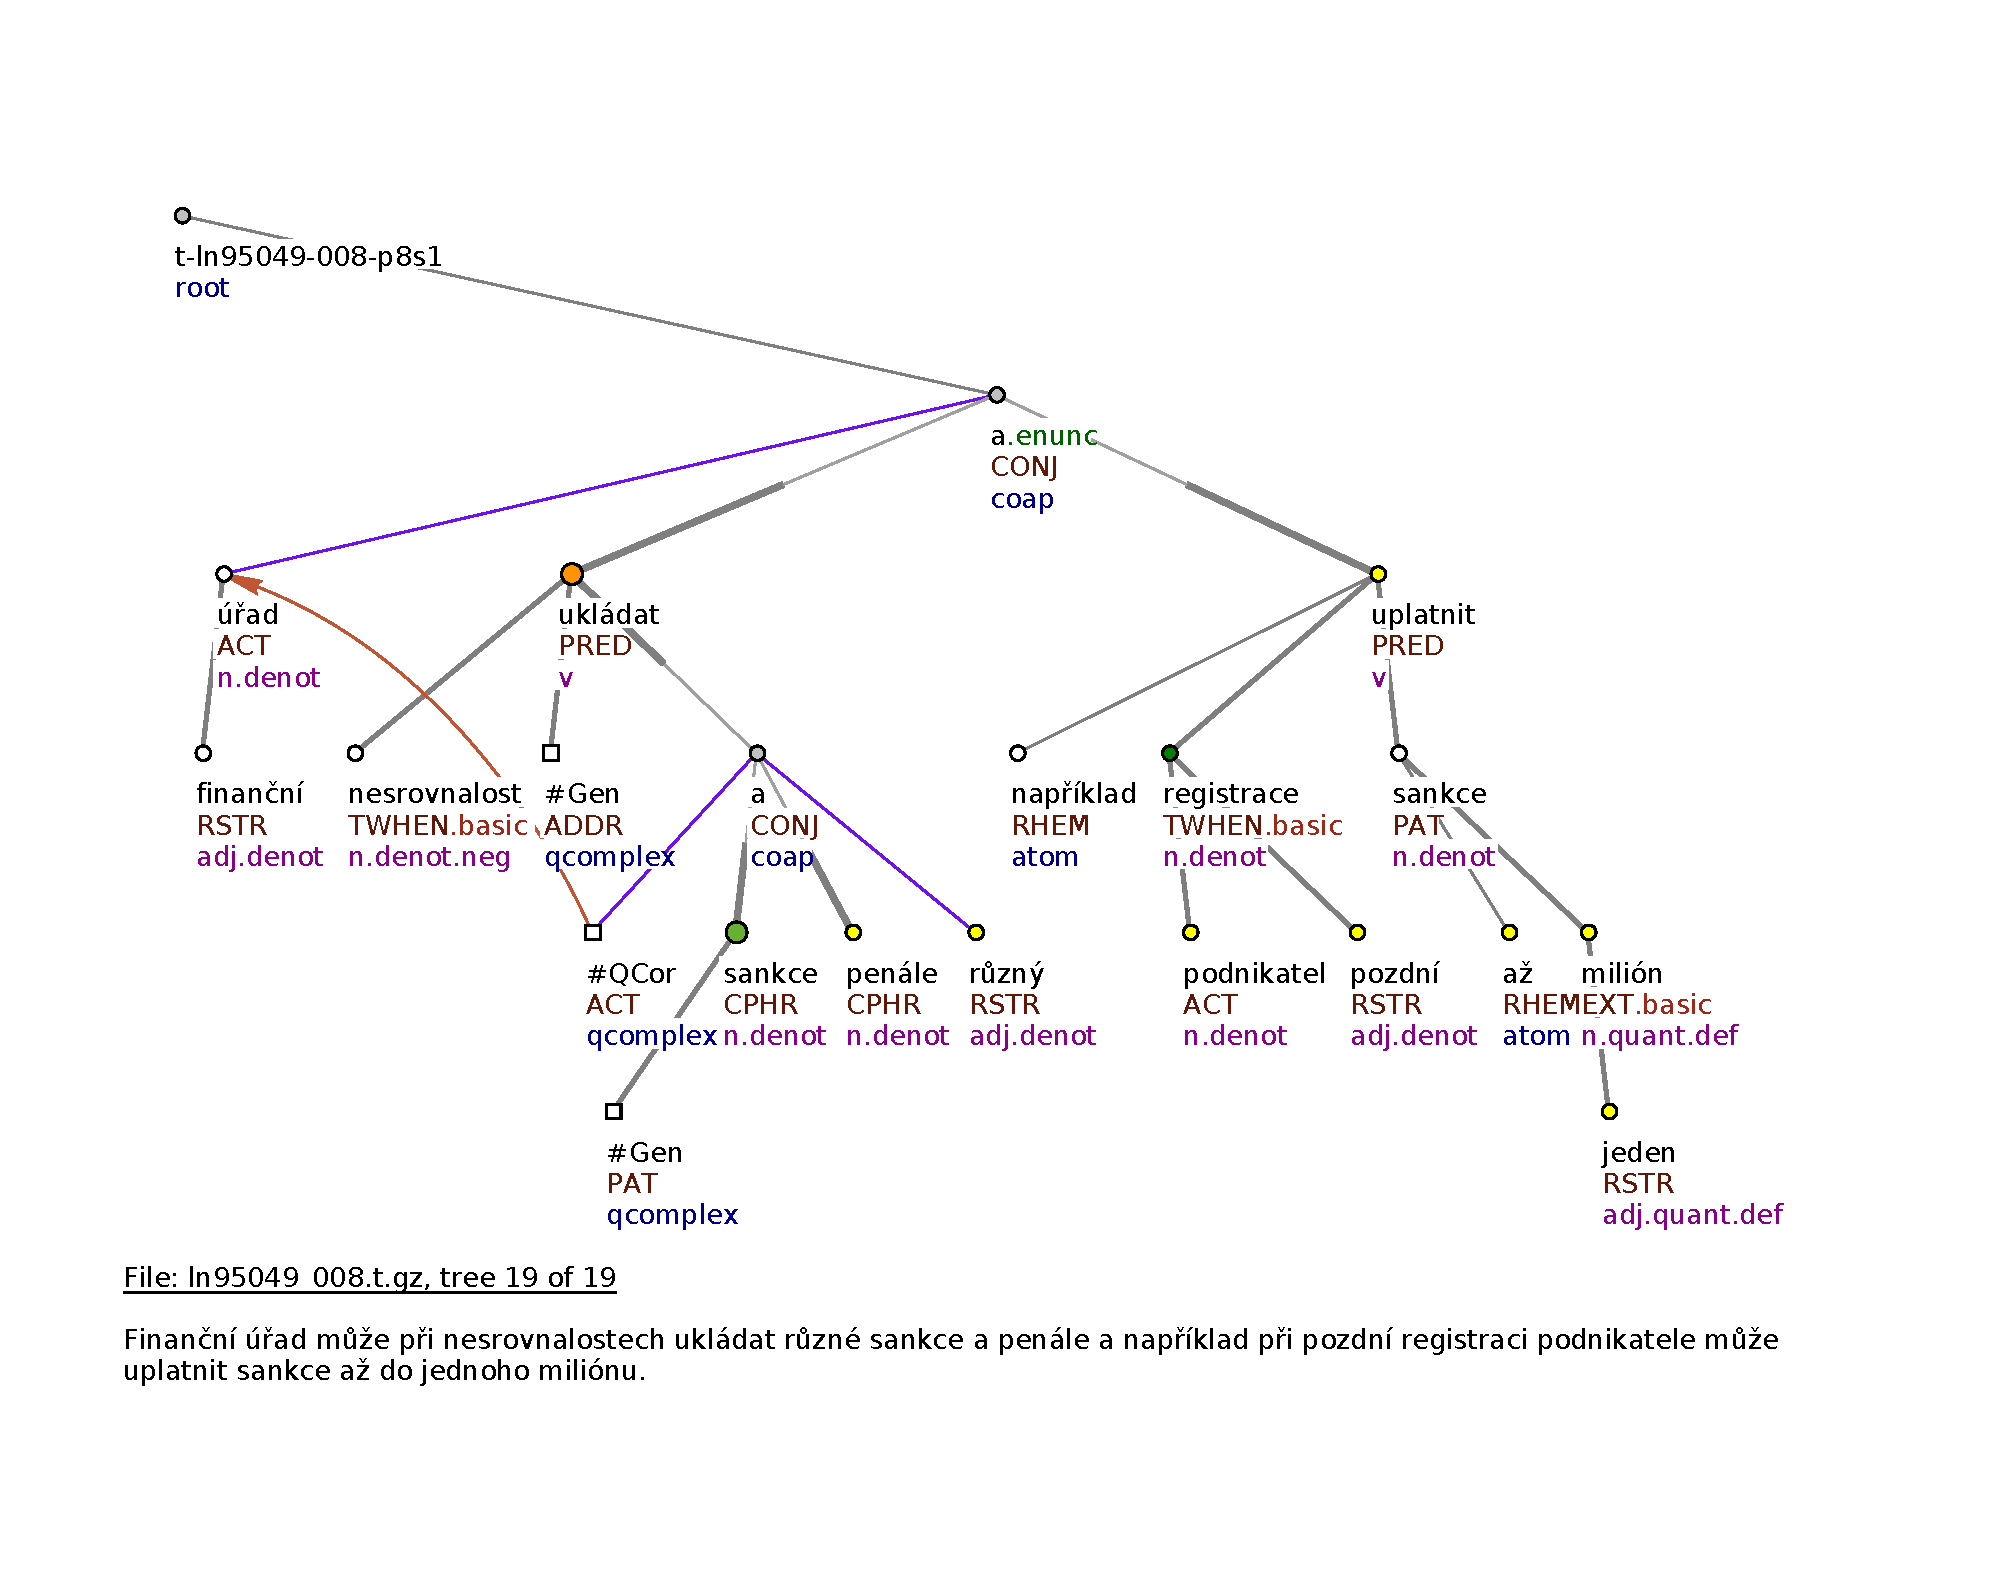
\includegraphics[width=\textwidth]{images/vyhledavky/cphr-ukladat-sankce-a-penale.pdf}
\caption{Coordination of two idioms starting with the same verb}
\label{fig:cphr-echild2}
\end{figure}

\newpage
\section{Notes}

{\em``Prokopnout pětku''} -- prokopnout [trestný kop after scoring] pětka -- ellipsis crossing into pragmatics(?), because it is {\em not} an ellipsis of some exact linguistic construction, but rather an ellipsis of a situation which everyone in the discourse understand.  

``Návrh / novela Zákona na ochranu osobních údajů''  $$((\mathrm{návrh} \lor \mathrm{novela}) | \mathrm{zákon} \lor \mathrm{předpis})$$
-- lexikální funkce?? \citep{wanner} ?

\subsection{Missing t-nodes in \code{coord}s}
``\textit{První} a druhá světová válka'' apod. -- the word ``První'' is an ellipsis of ``První světová válka''. The ellided t-nodes that should had been newly established were not, however, which left us two options, either annotate a single-word (and single-node) expression as an instance of a multi-word lexeme, or annotate the words ``světová válka'' that occure in the text as being a part of both expressions. We decided for the first, because the agreement on ellipses is fairly high in this type of coordinations.

% !TEX root = ../disertace.tex
%!TEX encoding = UTF-8 Unicode

\chapter{\sdata}
\section{The design and the PML schema}
\sdata\ means s-layer PML files and the PML schema of these files. The idea behind \sdata\ design is to have a simple way to store additional ``sense'' annotations over any layer of PDT. The annotations are stored as a set of ``sense'' nodes. Each s-node contains a link to a sense repository (annotation lexicon) and a set of references to nodes (m-, a- or t-) that correspond to an instance of the sense. An \sf\ is thus basically a very simple flat list of \sn{}s. It does not contain any trees. A single \sf\ can only reference a single PDT file: either tectogrammatical, or analytical, or even morphological layer can be used, but references to different layers cannot be mixed in one s-file.

The design of \sdata\ is quite universal. S-files can be used to provide additional annotations over any PML files that contain nodes with IDs. The sense repository (annotation lexicon) can be any dictionary that provides IDs for the entries. The tools used in our annotations mostly expect PDT PML or the particular \sf{}s that we have used, but that is mostly for convenience. Should the need appear to adapt the workflow a different corpus represented by PML files and a different annotation lexicon, the changes required would be rather minor.

\section{Visualisation}
There are two basic ways to view st-nodes: in \seman\ or in \tred. Both of these need to use the ``t-a-m-w-'' PDT files to display the sentence and/or the tree for each sentence and then they read the \stf\ to add the information about \stn{}s. The \stn{}s are displayed as colour boxes or bubbles over the words in a sentence or nodes in a tree in \seman\ or \tred\ respectively.

\subsection{Visualisation using \seman}
The visualisation of annotated files in \seman\ has the advantage of showing whole text with all the \mwe{}s clearly marked in a single glance. Integration of the SemLex browser is also beneficial, because it allows fast and convenient lookup of annotated \mwe{}s in \seman. Details of \seman\ interface are described in \Sref{sec:seman}. 

There are, however, also some drawbacks of this ``full plain text of an article'' approach: 

\section{\tred\ extension}
\tred\ has a powerful mechanism that allows it to be extended for new tasks. We developed an extension \texttt{pdt-t-st} that allows to see MWEs as graphically marked groups of tectogrammatical nodes. 

 Main features of the extension:
 \begin{itemize}
\item
Merges the \stf{}s into \tf{}s and allows to display these enriched tectogrammatical trees.
\item
Types of annotated MWEs (i.e. types of NEs and \semlex\ entries) are distinguished with the same colours that were used in \seman\ during annotations. This allows not only for easily seeing NE types, but also easily spotting annotators' disagreement on them. 
\item
Allows to merge annotations of several annotators into one \tf. 
\item
Each annotator's MWEs have a unique raster. It is thus easy to spot annotators' partial or full disagreement not on types of MWEs, but also on their spans.
\end{itemize}

 There are two ways to merge the \sdata\ and \tdata: 
 \begin{enumerate}
\item
Merge on opening the \stf\ in \tred, and
\item
Static merge that produces the merged \verb=*.t.mwe.gz= file. 
\end{enumerate}
The dynamic merging is done using a newly developed feature of \tred\footnote{Developed by Petr Pajas} that allows to apply arbitrary perl transformations on the input data. Thus we open the \stf, use the mechanism of extensions to activate our extension by identifying the \stf\ as data the extension can process and call our transformation. The transformation requires a \tf\ annotated by this \sf\ to be present in the same directory. The \tf\ and \sf\ are parsed, and for each \stn\ we find a tectogrammatical tree that includes \tn{}s annotated (i.e. referenced) in this \stn. When we have a root of the correct t-tree, the \stn{}s are basically added into an attribute \texttt{mwes} of this t-root. The attribute is rather complex, because it contains lists of \stn{}s for all annotators that annotated any \stn{}s in this tree. Some small transformations of \stn{}s are needed, as well as creation of some new XML nodes, to represent the information from \sf{}s in the \tf{}s properly. For all the details inspect the code of \verb=$pdt_t_st/libs/SDataMerge.pm=.
\bibliographystyle{plainnat}
\end{document}